\section*{Bài tập 02}

\subsection*{Dữ liệu ($10$ mẫu)}

\begin{center}
\small
\begin{tabular}{rcccccc}
ID & Tuổi & Lương & Điểm & Giới tính & Mua hàng\\\hline
1 & $25$ & $8000$ & $7{,}5$ & Nam & Yes \\
2 & $30$ & $?$ & $8{,}0$ & Nữ & No \\
3 & $22$ & $5000$ & $6{,}5$ & Nam & Yes \\
4 & $40$ & $15000$ & $9{,}0$ & Nữ & Yes \\
5 & $35$ & $-2000$ & $7{,}0$ & Nam & No \\
6 & $?$ & $7000$ & $6{,}0$ & Nữ & Yes \\
7 & $29$ & $8500$ & $8{,}5$ & Nam & Yes \\
8 & $50$ & $30000$ & $9{,}5$ & Nữ & Yes \\
9 & $27$ & $8200$ & $?$ & Nam & No \\
10 & $31$ & $7800$ & $7{,}8$ & Nữ & Yes \\
\end{tabular}
\end{center}

\subsubsection*{Câu 1}

Có $10$ quan sát (hàng) và $6$ cột (ID và năm thuộc tính). Nếu coi ID chỉ là mã dòng, còn $5$ thuộc tính dùng cho mô hình: Tuổi, Lương, Điểm là \emph{định lượng}; Giới tính là \emph{định tính} (danh mục); Mua hàng là nhãn nhị phân (Yes/No).

\subsubsection*{Câu 2}

Chỉ tính trên ô có số (bỏ quan sát thiếu từng cột).

\medskip
\textbf{Tuổi} ($9$ ô: bỏ ID $6$). Tổng $289$, trung bình $\bar x=289/9\approx 32{,}11$. Sắp tăng: $22,25,27,29,30,31,35,40,50$ --- trung vị (vị trí thứ $5$) là $30$. Mọi giá trị đều xuất hiện một lần nên \emph{không có mốt} theo nghĩa thống kê cổ điển.

\medskip
\textbf{Lương} ($9$ ô: bỏ ID $2$). Gồm cả $-2000$ (ID $5$). Tổng $87400$, trung bình $\approx9722{,}22$. Sắp tăng: $-2000,5000,7000,7800,8000,8200,8500,15000,30000$ --- trung vị $=8000$. Mốt: không có mốt cổ điển (một lần mỗi giá trị); giá trị $-2000$ về nội dung là sai lỗi, không nên diễn giải như mốt.

\medskip
\textbf{Điểm} ($9$ ô: bỏ ID $9$). Tổng $69{,}8$, trung bình $\approx 7{,}756$. Sắp tăng:
$6{,}0$, $6{,}5$, $7{,}0$, $7{,}5$, $7{,}8$, $8{,}0$, $8{,}5$, $9{,}0$, $9{,}5$ --- trung vị $=7{,}8$. Không có mốt cổ điển (mọi tần bằng $1$).

\subsubsection*{Câu 3}

Vẽ histogram cho Tuổi (chỉ các ô không thiếu) và boxplot cho Lương (các ô lương không trống, $-2000$ vẫn là một điểm). Minh họa:

\begin{center}
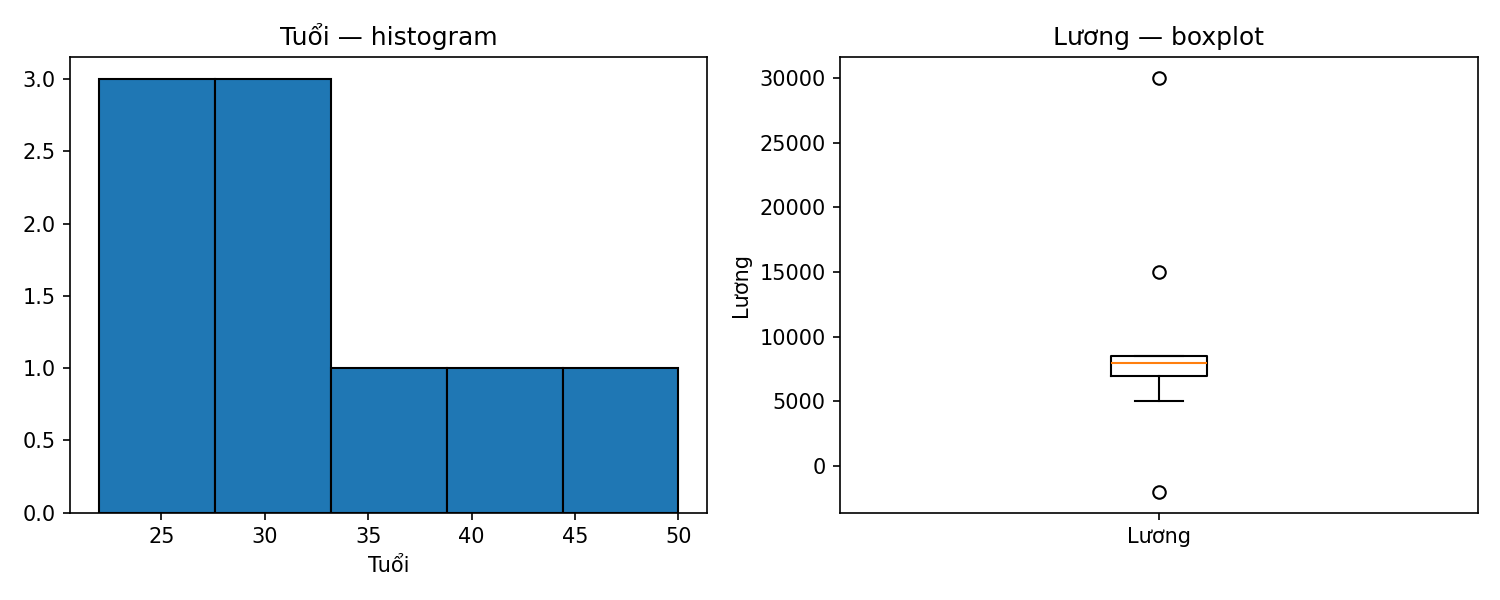
\includegraphics[width=\textwidth]{hist_tuoi_boxplot_luong_baitap02.png}
\end{center}

Hệ số bất đối xứng mẫu của Tuổi $\approx1{,}20>0$ --- phân bố Tuổi \emph{lệch phải} (đuôi về phía tuổi lớn). Boxplot Lương: có đuôi dài phía giá trị lớn và có điểm $-2000$ nằm xa phần còn lại --- vừa là điểm bất thường về \emph{nội dung} (lương âm).

\subsubsection*{Câu 4}

\begin{center}
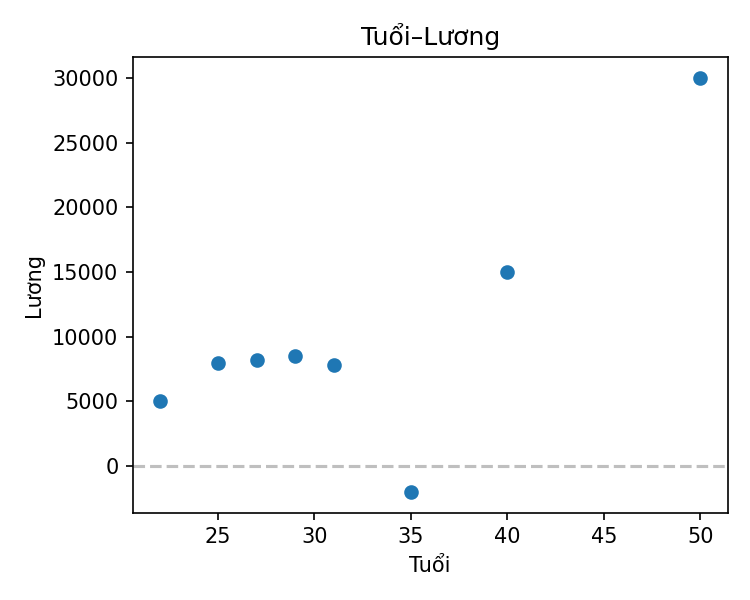
\includegraphics[width=0.55\textwidth]{scatter_age_luong_baitap02.png}
\end{center}

Trên $8$ cặp (Tuổi, Lương) đồng thời không thiếu, hệ số tương quan Pearson mẫu $r\approx0{,}75$ --- xu hướng \emph{dương} (tuổi tăng thì lương có xu hướng tăng), nhưng còn điểm lệch (ví dụ $-2000$). Gợi ý tiền xử lý: điền thiếu; xử lý lỗi $-2000$ (coi missing hoặc thay bằng giá trị đại diện sau khi làm sạch); có thể biến đổi sau khi lương đã dương và ổn định.

\subsubsection*{Câu 5}

Thiếu: Tuổi tại ID $6$ ($1/10=10\%$); Lương tại ID $2$ ($10\%$); Điểm tại ID $9$ ($10\%$). Ảnh hưởng: giảm số cặp đầy đủ cho tương quan; một số phương pháp không chấp nhận ô trống. Xử lý: điền thống kê hoặc mô hình đơn/đa biến; hoặc loại bản ghi nếu được phép.

\subsubsection*{Câu 6}

Trước khi điền: coi lương âm là không hợp lệ cho bước thống kê --- gán thành thiếu cho mục đích tính mean/median điền (để $-2000$ không kéo trung bình điền vào chỗ trống).

Hai cách điền phổ biến (sau bước trên). Với \emph{trung bình cột}, ví dụ Lương tại ID $2$ được điền $\approx11187{,}5$; Tuổi và Điểm cũng thay đổi so với median. Dưới đây là toàn bộ bảng sau \emph{điền bằng trung vị}:

\begin{center}
\small
\begin{tabular}{rccc}
ID & Tuổi & Lương & Điểm\\\hline
1 & $25$ & $8000$ & $7{,}5$ \\
2 & $30$ & $8100$ & $8{,}0$ \\
3 & $22$ & $5000$ & $6{,}5$ \\
4 & $40$ & $15000$ & $9{,}0$ \\
5 & $35$ & $8100$ & $7{,}0$ \\
6 & $30$ & $7000$ & $6{,}0$ \\
7 & $29$ & $8500$ & $8{,}5$ \\
8 & $50$ & $30000$ & $9{,}5$ \\
9 & $27$ & $8200$ & $7{,}8$ \\
10 & $31$ & $7800$ & $7{,}8$ \\
\end{tabular}
\end{center}

\emph{Chọn median:} dữ liệu Lương lệch và có giá trị cực lớn; trung vị bền hơn trung bình khi điền thiếu.

\subsubsection*{Câu 7}

Giá trị không hợp lệ: Lương $=-2000$ tại ID $5$ (không thực tế). Cách xử lý: đánh dấu missing rồi điền; hoặc thay bằng trung vị các lương dương sau khi kiểm tra --- nhất quán với Câu 6--9 bên dưới.

\subsubsection*{Câu 8}

Trên các ô Lương không trống trong bảng gốc: $Q_1=7000$, $Q_3=8500$, $\mathrm{IQR}=1500$, khoảng Tukey $[4750;\,10750]$. Các giá trị ngoài khoảng: $-2000$, $15000$, $30000$.

Chuẩn hóa $z_i=(x_i-\mu)/\sigma$ với $\mu$, $\sigma$ mẫu trên các lương không thiếu ($\mu\approx9722$, $\sigma\approx8277$). Với ngưỡng $|z|>3$ không có điểm nào; tuy vậy $-2000$ và $30000$ vẫn là ngoại lai mạnh theo IQR và cần xử lý theo Câu 7.

\subsubsection*{Câu 9}

Sau khi điền thiếu bằng \emph{trung vị} (như Câu 6) và thay lương âm bằng trung vị các lương dương ($8100$), chuẩn hóa Z-score cột Lương:
\[
z=\frac{x-\mu}{\sigma}
\]
(ước lượng $\mu,\sigma$ trên $10$ giá trị sau làm sạch). Giá trị:

\begin{center}
\small
\begin{tabular}{rcc}
ID & Lương (sau xử lý) & $z$\\\hline
1 & $8000$ & $-0{,}371995$ \\
2 & $8100$ & $-0{,}357520$ \\
3 & $5000$ & $-0{,}806230$ \\
4 & $15000$ & $0{,}641221$ \\
5 & $8100$ & $-0{,}357520$ \\
6 & $7000$ & $-0{,}516740$ \\
7 & $8500$ & $-0{,}299622$ \\
8 & $30000$ & $2{,}812397$ \\
9 & $8200$ & $-0{,}343046$ \\
10 & $7800$ & $-0{,}400944$ \\
\end{tabular}
\end{center}

Trung bình các $z$ gần $0$ và độ lệch chuẩn gần $1$: đổi thang đo Lương sang đơn vị ``số sigma'' để so sánh cùng thang với các thuộc tính khác sau này.

\subsubsection*{Câu 10}

One-hot giới tính: hai cột nhị phân tương ứng Nam và Nữ (Nam $\to(1,0)$, Nữ $\to(0,1)$). Mua hàng nhị phân: Yes $\to1$, No $\to0$.

\begin{center}
\small
\begin{tabular}{rrrrrrr}
ID & Tuổi & Lương & Điểm & Nam & Nữ & Mua\\\hline
1 & 25 & 8000 & 7{,}5 & 1 & 0 & 1 \\
2 & 30 & 8100 & 8{,}0 & 0 & 1 & 0 \\
3 & 22 & 5000 & 6{,}5 & 1 & 0 & 1 \\
4 & 40 & 15000 & 9{,}0 & 0 & 1 & 1 \\
5 & 35 & 8100 & 7{,}0 & 1 & 0 & 0 \\
6 & 30 & 7000 & 6{,}0 & 0 & 1 & 1 \\
7 & 29 & 8500 & 8{,}5 & 1 & 0 & 1 \\
8 & 50 & 30000 & 9{,}5 & 0 & 1 & 1 \\
9 & 27 & 8200 & 7{,}8 & 1 & 0 & 0 \\
10 & 31 & 7800 & 7{,}8 & 0 & 1 & 1 \\
\end{tabular}
\end{center}

(Các cột số Tuổi, Lương, Điểm ở đây trùng với bảng sau khi điền median và thay lương âm như Câu 6--9.)

\subsubsection*{Câu 11}

\begin{itemize}
  \item \textbf{ID:} bỏ khỏi tập đặc trưng dự báo (chỉ là chỉ số, dễ gây học nhầm nếu mô hình quá phức tạp).
  \item \textbf{Tuổi, Lương, Điểm:} giữ sau khi xử lý thiếu/lỗi; đây là thông tin hữu ích cho Mua hàng.
  \item \textbf{Giới tính:} giữ dưới dạng one-hot như Câu 10.
  \item Cột nhiều missing/lỗi chưa xử lý sẽ làm giảm chất lượng --- cần làm sạch trước hoặc giảm trọng số trong phân tích.
\end{itemize}

\subsubsection*{Câu 12}

Với chỉ vài biến định lượng và mẫu nhỏ, \emph{giảm chiều đơn giản} (bỏ ID, có thể gộp biến nếu tương quan quá cao sau khi làm sạch) thường đủ.

\emph{PCA} phù hợp khi có nhiều biến định lượng tương quan cao và cần nén xuống vài thành phần --- nên \emph{chuẩn hóa} trước PCA. Ở bài này số chiều định lượng ít và còn biến danh mục; PCA không bắt buộc trừ khi sau này bổ sung nhiều cột liên quan (ví dụ nhiều loại điểm số hoặc chỉ số tổng hợp).
